\chapter{Referencial Teórico}
\label{cap:fundamentacao-teorica}

Visando dar o entendimento a parte do material que serviu como inspiração e aprofundamento para os conhecimentos a serem descritos neste trabalho, seguem a seguir 

\section{APQP}

O \  \gls{APQP} é um método estruturado para definir e estabelecer as etapas necessárias para garantir que um produto satisfaça as necessidades e expectativas do cliente . O objetivo do mesmo é facilitar a comunicação e a colaboração entre todas as partes envolvidas no desenvolvimento do produto, desde o planejamento até a produção  \cite{apqp}.

Desenvolvido no início dos anos 1990 pelas montadoras automotivas General Motors, Ford e Chrysler nos Estados Unidos. Essas empresas perceberam a necessidade de um processo padronizado para garantir a qualidade do produto desde o início do processo de desenvolvimento. O  \gls{APQP} consiste em cinco fases principais:

\begin{figure}
    \centering
    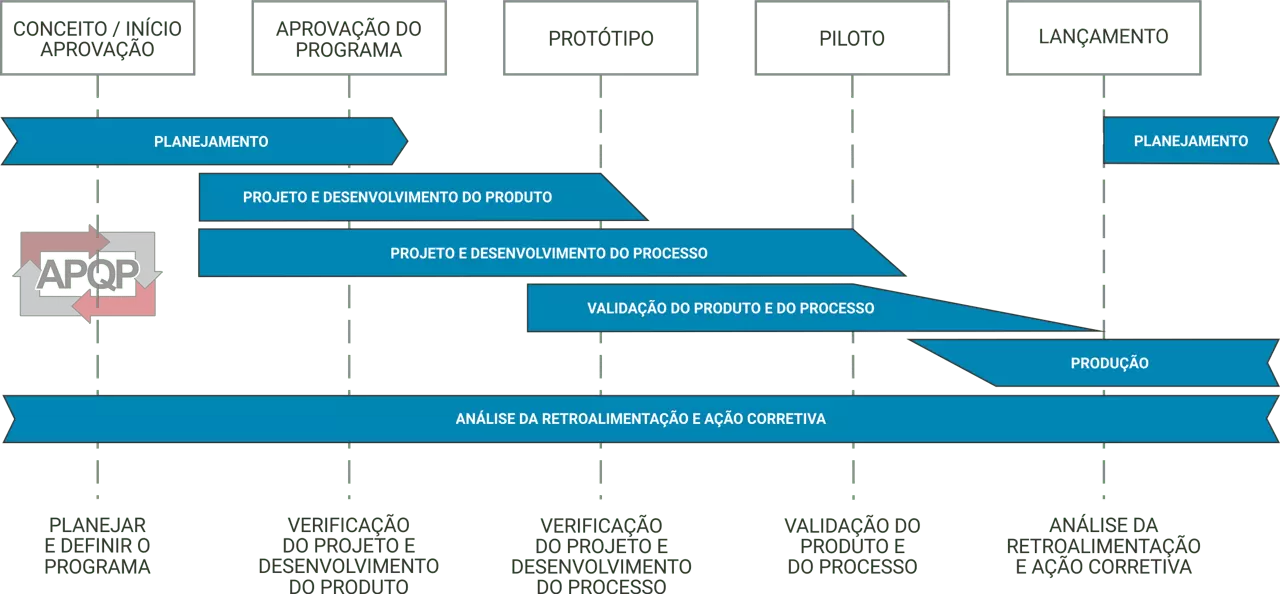
\includegraphics[width=0.5\linewidth]{figuras/total.png}
    
    \label{fig:enter-label}
    		\Fonte{Captura de tela do site \cite{apqp}{}}
\end{figure}

\begin{enumerate}
    \item Planejamento e Definição do Programa: Nesta fase, são definidos os objetivos do programa, os requisitos do cliente e a equipe responsável pelo desenvolvimento do produto.
    \item Projeto e Desenvolvimento do Produto: Aqui, ocorre o desenvolvimento do projeto do produto, incluindo a definição de requisitos, desenhos, especificações e protótipos.
    \item Projeto e Desenvolvimento do Processo: Nesta fase, o foco está no desenvolvimento do processo de fabricação do produto, incluindo a definição dos métodos de produção, equipamentos, ferramentas e controle de qualidade.
    \item Validação do Produto e Processo: É realizada a validação do produto e do processo, por meio de testes, análises e verificações para garantir que o produto atenda aos requisitos do cliente.
    \item \textit{Feedback} do Cliente e Ações Corretivas: Nesta última fase, é feita a avaliação do desempenho do produto no mercado e o \textit{feedback} dos clientes. Com base nisso, são identificadas ações corretivas para melhorar a qualidade do produto.
\end{enumerate}

O sistema é amplamente utilizado na indústria automotiva, mas também pode ser aplicado em outros setores que buscam garantir a qualidade do produto desde o início do processo de desenvolvimento. Ele envolve a utilização de diversas ferramentas e metodologias, como \gls{FMEA}, \gls{PPAP}, \gls{CEP}, \gls{MSA}, para garantir a qualidade do produto em todas as etapas do processo  \cite{apqp}.

\section{Usabilidade}

A usabilidade, refere-se à capacidade de um produto, sistema ou serviço ser utilizado de maneira eficaz, eficiente e satisfatória pelos seus usuários \cite{iso20199241}. A ISO adverte sobre a importância de projetar produtos que sejam fáceis de aprender e utilizar, levando em consideração as características e necessidades dos usuários. 

Pode ainda ser avaliada com base em critérios como a facilidade de aprendizado, a eficiência de uso, a facilidade de memorização, a taxa de erros, a satisfação do usuário e outros aspectos relacionados à interação entre o usuário e o produto \cite{betiol2010ergonomia}. Os autores também abordam métodos e técnicas para avaliar a usabilidade, como testes com usuários, avaliação heurística e análise de tarefas.

\section{Efeito estética na usabilidade}

Usuários tendem a perceber produtos com design esteticamente agradável como mais utilizáveis e confiáveis. Ou seja, a aparência visual de um produto pode impactar a forma como os usuários o percebem e interagem com ele. \cite{norman2008design}

No entanto, é importante ressaltar que a estética não deve ser considerada apenas como um fator isolado, mas sim em conjunto com outros princípios de usabilidade, como facilidade de uso, eficiência e satisfação do usuário \cite{kurosu1995apparent} . Um produto com ótima aparência, mas difícil de usar, pode causar frustração e insatisfação.

Portanto, ao projetar produtos ou interfaces, é importante considerar tanto a estética quanto a usabilidade, buscando encontrar um equilíbrio entre uma aparência atraente e uma experiência de uso eficiente e intuitiva.

\section{Método de coleta de dados}

\subsection{\textbf{\textit{Benchmarking}}}

É um processo essencial que envolve a comparação e análise de produtos, serviços e práticas empresariais de outras organizações para identificar as melhores abordagens e referências que possam ser aplicadas para melhorar o desempenho e a eficiência de um negócio. Trata-se de uma ferramenta de gestão valiosa que permite às empresas aprender com seus concorrentes e outras organizações líderes, identificar oportunidades de aprimoramento e implementar mudanças para alcançar um desempenho superior.

Durante o processo de \textit{benchmarking}, as empresas selecionam cuidadosamente seus concorrentes ou referências em setores relacionados e estabelecem indicadores de análise para comparar aspectos específicos, tanto qualitativos quanto quantitativos. A pesquisa é uma etapa fundamental, envolvendo a coleta de informações a partir de diversas fontes, como relatórios de mercado, estudos exploratórios, entrevistas e revisão bibliográfica.

Uma vez que os dados são coletados, eles passam por uma análise minuciosa das práticas das empresas de referência, com a compilação e interpretação das informações para chegar a conclusões e identificar pontos fortes e fracos \cite{rogers2013design}. O \textit{benchmarking} possibilita a identificação clara de áreas que precisam de aprimoramento, a medição do progresso ao longo do tempo e a tomada de decisões mais embasadas.

\subsection{\textbf{Entrevista}}

Essa técnica de pesquisa qualitativa é amplamente utilizada para compreender as necessidades, expectativas, experiências e opiniões dos usuários em relação a sistemas interativos\cite{rogers2013design}.

Durante a entrevista em \gls{IHC}, o pesquisador utiliza perguntas abertas para explorar a perspectiva do usuário sobre a \gls{UI}, sua usabilidade, eficácia e satisfação. O objetivo é obter \textit{insights} valiosos que possam ser aplicados no processo de design e desenvolvimento de interfaces mais eficientes e satisfatórias para os usuários \cite{barbosa2021interaccao} .

As entrevistas em \gls{IHC} podem ser conduzidas individualmente, em grupo ou em contexto natural de uso, dependendo do objetivo da pesquisa e das características do público-alvo. Elas são geralmente guiadas por um roteiro de perguntas, que pode ser estruturado, semi-estruturado ou não estruturado, dependendo do nível de controle que o pesquisador deseja ter sobre a entrevista \cite{barbosa2021interaccao}.

Através das entrevistas, os pesquisadores podem identificar problemas de usabilidade, descobrir necessidades e expectativas dos usuários, identificar pontos de melhoria e obter \textit{feedback} valioso para o aprimoramento contínuo das \gls{UI}. As informações coletadas durante as entrevistas são analisadas e utilizadas para informar o processo de design e desenvolvimento, garantindo que as interfaces atendam às necessidades e expectativas dos usuários.

\subsection{\textbf{Levantamento e análise de requisitos}}

Um levantamento de requisitos é o processo de identificação e compreensão das necessidades e expectativas do cliente em relação a um sistema de software que será desenvolvido \cite{mach}. Durante essa etapa, são coletadas informações sobre as funcionalidades, características e restrições do sistema, a fim de definir claramente o que o software deve fazer e como deve atender às necessidades do usuário.

Durante o processo de levantamento de requisitos , podem ser utilizadas diversas técnicas, como entrevistas com os usuários, questionários, observação do ambiente de trabalho, análise de documentos e prototipagem \cite{rogers2013design}. Essas técnicas ajudam a obter informações precisas e detalhadas sobre as necessidades do cliente e a garantir a qualidade dos requisitos levantados.

\section{Lei de Tesler }
A Lei de Tesler, também conhecida como Lei da Conservação da Complexidade , é uma das leis de \gls{UX} que afirma que a complexidade de um sistema nunca desaparece , ela apenas muda de lugar e impacta outros agentes \cite{yablonski2020leis}. Essa lei propõe que, ao simplificar um recurso de uma \gls{UI} , a complexidade migra para os desenvolvedores ou outros componentes do sistema.

Ao simplificar uma parte da interface para torná-la mais fácil de usar para o usuário, é necessário que os desenvolvedores assumam a complexidade e a mantenham nos bastidores do sistema. Essa lei destaca o fato de que a complexidade não pode ser totalmente eliminada, mas pode ser gerenciada e distribuída de maneira mais eficiente.

A Lei de Tesler é importante no design de interfaces, pois ajuda a equilibrar a simplicidade para os usuários com a complexidade necessária para o funcionamento do sistema. Os profissionais de \gls{UX} devem considerar cuidadosamente quais elementos da \gls{UI} devem ser simplificados e quais complexidades devem ser gerenciadas pelos desenvolvedores, a fim de fornecer uma experiência do usuário eficaz e satisfatória.

\section{Técnica de prototipagem}

A prototipagem é o processo de criação de um modelo ou representação inicial de um produto, sistema ou interface antes de ser desenvolvido completamente. As técnicas de prototipagem são os métodos e abordagens usados para criar esses protótipos. Existem várias técnicas de prototipagem disponíveis, que podem ser usadas de acordo com as necessidades e recursos disponíveis. Algumas das técnicas comuns de prototipagem incluem prototipagem de papel, prototipagem digital, prototipagem 3D, prototipagem de alta fidelidade e iterativa

Cada técnica de prototipagem tem suas vantagens e desvantagens, e a escolha da técnica adequada depende do contexto do projeto, dos recursos disponíveis e dos objetivos específicos do protótipo.

\section{Lei de Jakob }

A Lei de Jakob, também conhecida como Lei da Familiaridade ou Lei da Experiência Acumulada, é uma das leis de \gls{UX} que afirma que os usuários preferem interfaces que são familiares e consistentes com aquelas que já conhecem \cite{yablonski2020leis}.

De acordo com a lei proposta, os usuários passam a maior parte do tempo em outros sites ou aplicativos , o que significa que eles têm um repertório de experiências previamente acumuladas nesses produtos. Portanto, é natural que eles prefiram que um novo produto funcione de forma semelhante aos outros que já conhecem.

Essa preferência não se deve apenas a uma questão de gosto pessoal , mas também é baseada em observações matemáticas sobre a curva de aprendizado . Quanto mais familiar um usuário estiver com uma interface, mais rápido ele será capaz de realizar uma tarefa, pois já conhece os padrões e as interações.

Nielsen ainda destaca a importância da consistência no d\gls{UI}. Ao seguir padrões e convenções estabelecidos, os designers podem criar interfaces que sejam intuitivas e fáceis de usar para os usuários, minimizando a curva de aprendizado e aumentando a eficiência.

\section{Lei de Hick }

A Lei de Hick, ou Lei de Hick-Hyman, é uma lei da psicologia cognitiva que descreve o tempo que uma pessoa leva para tomar uma decisão com base no número de opções disponíveis \cite{yablonski2020leis}.

De acordo com a proposição , quanto mais opções são apresentadas a uma pessoa, mais tempo ela levará para tomar uma decisão. Isso ocorre porque o cérebro humano precisa processar e analisar cada opção antes de fazer uma escolha. À medida que o número de opções aumenta, o tempo necessário para processar e tomar uma decisão também aumenta.

Essa lei é frequentemente aplicada no design de \gls{UI} e no campo de \gls{UX}. Os designers a usam para entender como a apresentação de opções pode afetar o tempo de tomada de decisão dos usuários . Em projetos de design, é comum buscar reduzir o número de opções e simplificar a interface para facilitar a tomada de decisão dos usuários

Em resumo, proposta de lei destaca o impacto do número de opções disponíveis na tomada de decisão dos usuários. Ao entender e aplicar essa lei, os designers podem criar interfaces mais eficientes e facilitar a experiência do usuário.

\section{Heurísticas de Nielsen}

As heurísticas de Nielsen, são um conjunto de diretrizes de design amplamente utilizadas no campo da usabilidade e (\gls{UX}) para avaliar e melhorar a qualidade das interfaces de usuário. As 10 heurísticas de Nielsen são as seguintes  \cite{nielsen1994usability}

\begin{enumerate}
    \item Visibilidade do status do sistema: O sistema deve sempre informar aos usuários o que está acontecendo, fornecendo \textit{feedback} adequado sobre suas ações.
    \item Correspondência entre o sistema e o mundo real : A linguagem, os conceitos e as convenções utilizadas na interface devem ser familiares e se alinhar com o mundo real dos usuários.
    \item Controle e liberdade do usuário: Os usuários devem ter a capacidade de desfazer ações indesejadas e explorar livremente a interface.
    \item Consistência e padrões: Elementos da interface devem ser consistentes e seguir padrões estabelecidos para facilitar o reconhecimento e a compreensão.
    \item Prevenção de erros: A interface deve ser projetada para evitar erros, fornecendo orientações claras e evitando condições propensas a erros.
    \item Reconhecimento em vez de recordação: Os usuários devem ser capazes de reconhecer opções e ações, em vez de ter que lembrar informações específicas.
    \item Flexibilidade e eficiência de uso: A interface deve ser projetada para acomodar diferentes níveis de habilidade e permitir que usuários experientes realizem tarefas de forma mais rápida.
    \item Estética e design minimalista: A interface deve ser visualmente agradável, com elementos visuais bem organizados e sem informações desnecessárias.
    \item Ajuda e documentação: A interface deve fornecer suporte e documentação adequada para ajudar os usuários a entender e utilizar o sistema.
    \item Reconhecimento de erro: Quando os usuários cometem erros, a interface deve fornecer mensagens claras, específicas e construtivas para ajudá-los a entender e corrigir os problemas.

\end{enumerate}

Essas heurísticas são consideradas princípios fundamentais para \gls{UI} eficazes e usáveis. Ao seguir essas diretrizes, os designers podem criar interfaces mais intuitivas, fáceis de usar e que atendam às necessidades dos usuários.